\documentclass{article}  % Define la clase del documento.

% Paquetes de idioma y codificación
\usepackage[utf8]{inputenc}
\usepackage[T1]{fontenc}
\usepackage[spanish]{babel}  % Ajusta el idioma del documento a español.

% Paquete de geometría para configurar márgenes y tamaño de papel
\usepackage[letterpaper, margin=3cm]{geometry}

% Paquetes de tipografía
\usepackage{mathptmx}    % Usa Times New Roman como fuente.
\usepackage{microtype}   % Mejora la justificación del texto.

% Paquetes para manejo de colores y gráficos
\usepackage{xcolor}      % Define y utiliza colores.
\usepackage{graphicx}    % Permite la inserción de imágenes.
\usepackage{tikz}        % Creación de gráficos vectoriales.

% Configuración de enlaces y referencias cruzadas
\usepackage{hyperref}
\hypersetup{
    colorlinks   = true,
    linkcolor    = darkblue,
    citecolor    = black,
    filecolor    = blue,
    urlcolor     = blue
}

% Paquetes para la mejora visual de tablas y figuras
\usepackage{booktabs}    % Para tablas de alta calidad.
\usepackage{float}       % Controla la posición de figuras y tablas.

% Paquete para la personalización de códigos fuente
\usepackage{listings}
\lstset{
    literate=
    {á}{{\'a}}1 {é}{{\'e}}1 {í}{{\'i}}1 {ó}{{\'o}}1 {ú}{{\'u}}1
    {Á}{{\'A}}1 {É}{{\'E}}1 {Í}{{\'I}}1 {Ó}{{\'O}}1 {Ú}{{\'U}}1
    {ñ}{{\~n}}1 {Ñ}{{\~N}}1 {ü}{{\"u}}1 {Ü}{{\"U}}1,
    backgroundcolor=\color{backcolour},
    commentstyle=\color{codegreen},
    keywordstyle=\color{codepurple},
    numberstyle=\tiny\color{codegray},
    stringstyle=\color{red},
    basicstyle=\ttfamily\small,
    breakatwhitespace=false,
    breaklines=true,
    captionpos=b,
    keepspaces=true,
    numbers=left,
    numbersep=5pt,
    showspaces=false,
    showstringspaces=false,
    showtabs=false,
    tabsize=2,
    language=TeX,
    morecomment=[l]\#,
    frame=single,
    rulecolor=\color{black}
}

% Definición de colores al estilo Visual Studio Code
\definecolor{darkblue}{rgb}{0.0, 0.0, 0.55}  % Enlaces
\definecolor{codegreen}{rgb}{0.25, 0.49, 0.48}  % Comentarios
\definecolor{codegray}{rgb}{0.5, 0.5, 0.5}  % Números y anotaciones
\definecolor{codepurple}{rgb}{0.58, 0, 0.82}  % Palabras clave
\definecolor{backcolour}{rgb}{0.95, 0.95, 0.92}  % Fondo de código

% Configuraciones de párrafo y matemáticas
\usepackage{amsmath}
\usepackage{parskip}    % Espaciado entre párrafos.
\usepackage{ragged2e}   % Justificación mejorada.
\usepackage{graphicx} % Paquete necesario para incluir imágenes
\usepackage{subcaption} % Paquete necesario para incluir subfiguras

% Configuración de secciones y encabezados
\usepackage{titlesec}
\titleclass{\part}{top} % Make part like a class
\titleformat{\part}[display]
  {\normalfont\huge\bfseries\centering}{\thepart}{20pt}{\Huge}
\titlespacing*{\part}{0pt}{-60pt}{10pt}
\titleformat{\part}
  {\normalfont\huge\bfseries}{}{0pt}{}

% Asegúrate de usar esto para mantener el estilo en las páginas de las partes
\titleformat{\part}[display]
  {\normalfont\huge\bfseries}{}{0pt}{}
  [\thispagestyle{fancy}] % Aplica el estilo fancy a las páginas de las partes

% Configuración de encabezados y pies de página personalizados
\usepackage{fancyhdr}
\pagestyle{fancy}
\fancyhf{}
\fancyhead[L]{\raisebox{0.20cm}{\textbf{Apuntes Prueba 1 Hidrologia}}}
\fancyhead[R]{\raisebox{0.1cm}{
\includegraphics[width=0.25\linewidth]{LOGO_UNIVERSIDAD.jpg}}}
\fancyhead[C]{\rule{\textwidth}{0.6pt}}
\fancyfoot[C]{\rule{\textwidth}{0.6pt}}
\fancyfoot[R]{\raisebox{-1.5\baselineskip}{\thepage}}
\renewcommand{\headrulewidth}{0pt}
\renewcommand{\footrulewidth}{0pt}

% Configuración avanzada de geometría
\geometry{
  top=3.5cm, % Aumenta el espacio en la parte superior para subir el encabezado
  bottom=2.5cm,
  headheight=2.5cm % Aumenta la altura del encabezado si es necesario
}

% Configuracion de bibliografia
\usepackage{natbib}
\bibliographystyle{unsrtnat}  % Puedes cambiarlo por `unsrtnat`, `abbrvnat`, etc.

\begin{document}
%----------------------------------------------------------------------------------------
% PORTADA
%----------------------------------------------------------------------------------------
\begin{titlepage}%Inicio de la carátula, solo modificar los datos necesarios
\newcommand{\HRule}{\rule{\linewidth}{0.5mm}} 
\center 
%----------------------------------------------------------------------------------------
%	ENCABEZADO
%----------------------------------------------------------------------------------------

\includegraphics[width=10cm]{LOGO_UNIVERSIDAD.jpg}\\ % Si esta plantilla se copio correctamente, va a llevar la imagen del logo de la facultad.OBS: Es necesario incluir el paquete: graphicx
\vspace{3cm}
%----------------------------------------------------------------------------------------
%	SECCION DEL TITULO
%----------------------------------------------------------------------------------------
\HRule \\[0.4cm]
{ \huge \bfseries Apuntes Prueba 2}\\[0.4cm] % Titulo del documento
{ \huge \bfseries Métodos y técnicas de la construcción}\\[0.4cm] % Titulo del documento
\HRule \\[1.5cm]
 \vspace{5cm}
%----------------------------------------------------------------------------------------
%	SECCION DEL AUTOR
%----------------------------------------------------------------------------------------
\begin{flushright}
    { 
    \textbf{Autores:} \\
    Lukas Wolff Casanova\\
    Felipe Vicencio\\
    Berni\\
    Pedro?\\
}
\end{flushright}
\vspace{1cm}
%----------------------------------------------------------------------------------------
%	SECCION DE LA FECHA
%----------------------------------------------------------------------------------------
{\large \textbf{\today}}\\[2cm] % El comando \today coloca la fecha del dia, y esto se actualiza con cada compilacion, en caso de querer tener una fecha estatica, reemplazar el \today por la fecha deseada
\end{titlepage}
%----------------------------------------------------------------------------------------
%  INDICE
%----------------------------------------------------------------------------------------
\newpage
\thispagestyle{empty} % Deshabilita el número de página en la página del índice
\tableofcontents
\thispagestyle{plain} % Deshabilita el encabezado en la página del índice
\thispagestyle{empty} % Deshabilita el número de página en la página del índice
\newpage

%\newpage
%\thispagestyle{empty}
%\listoffigures 
%\thispagestyle{plain} % Deshabilita el encabezado en la página del índice %
%\thispagestyle{empty}
%\newpage
%----------------------------------------------------------------------------------------
%ACÁ EMPIEZA EL INFORME
\setcounter{page}{1}
%----------------------------------------------------------------------------------------
\part{Capítulo 4: Contratos y propuestas en proyectos de Construcción}

Es un convenio entre el que construye y el dueño o mandante que financia, y fija sus objetivos
de acuerdo con sus necesidades y posibilidades. El propósito de un contrato de construcción
es definir derechos, obligaciones y responsabilidades de cada una de las partes involucradas.
\\ \\
El propietario puede designar una inspección para controlar la obra. Es como intermediario entre
contratista y mandante. Hay contratos que le adjutican esta responsabilidad a un "Árbitro".

\begin{itemize}
    \item Modalidades de Contratos de construcción
    \begin{itemize}
        \item Construir para sí: Usa sus propios recursos para la ejecución de proyectos arriesgándose a la no aceptación de este por parte del mercado inmobiliario.
        \item Construir por terceros: Obra es financiada por el mandante, y el contratista ejecuta. Pueden tener las siguientes relaciones.
        \begin{itemize}
            \item Mandante entrega el proyecto y lo financia, contratista lo ejecuta.
            \item Mandante financia la obra, solicita el diseño y la ejecución al contratista.
            \item Contratista diseña, ejecuta y financia la obra y entrega la obra terminada al mandante en un precio previamente convenido (contrato llave en mano).
        \end{itemize}
    \end{itemize}
    \item Tipos de Contratos
    \begin{itemize}
        \item Contrato de suma alzada: Contratista realiza toda la obra a un precio fijo (propuesto por él después de estudiar el proyecto y aceptado por el mandante). Máximo riesgo es del contratista.
        \begin{itemize}
            \item Proyecto tiene que estar 100\% definido.
            \item Dueño escoge la mejor oferta.
            \item Los cambios son casi imposibles por parte del mandante, debido al contrato de adjudicación.
            \item Contratista debe hacer un análisis de costos precisos para dar la oferta.
        \end{itemize}
        \item Contrato de precios unitarios: Se establecen precios unitarios para cada partida de la obra, y se paga por la cantidad de trabajo realizado. Se paga por lo que se hace. El riesgo es compartido entre mandante y contratista. Es competitivo.
        \begin{itemize}
            \item Se puede ofertar sin tener el proyecto definido.
            \item Permite al dueño saber exactamente cuánto va a invertir en la obra.
            \item Contratista deberá realizar un estudio de costos preciso.
        \end{itemize}
        \item Contrato de administración delegada: Contratista se encarga de la administración de la obra, y el mandante paga los costos de la obra y un porcentaje adicional por la administración (honorarios). El riesgo es del mandante. Se recomienda como opción de emergencia y sin competencia, cuando se tiene completo el proyecto y se debe cumplir en un plazo corto. Se requiere confianza e inspecciones constantes.
        \begin{itemize}
            \item Dueño no conoce el presupuesto final.
            \item Contratista no corre riesgo con ganancias.
            \item Contratista puede encarecer la obra.
            \item Si los honorarios son fijos, contratista se motiva a terminar antes.
            \item Si honorarios tienen incentivo por horario/plazo, contratista se motiva a cumplir.
        \end{itemize}
    \end{itemize}
    \item Condiciones previas al llamado de una propuesta.
    \begin{itemize}
        \item Mandante debe tener claro lo que se quiere construir, el costo, el financiamiento y adicionales.
        \item Mandante debe informar al proyectista el costo aproximado de la obra.
        \item Mandante debe avisar al proyectista el tipo de contrato que se concretará.
        \item Incluir método constructivo en el diseño del proyecto.
        \item Se deben elaborar las bases administrativas por las que se regirá el contrato.
        \item Mandante podría encargar un estudio de presupuesto e inversión oficial de la obra. Se suele saltar esto.
        \item Establecer clara y rígidamente el sistema de pago que se implantará y la fuente de financiamiento de la obra.
        \item Elaborar el proyecto a cabalidad y en lo posible concertar una o más reuniones con todos los proyectistas participantes.
        \item Existen propuestas públicas (todos los que cumplan los requisitos) y privadas (aquellos invitados).
        \item OJO: El Estado está obligado por carta fundamental a llamar licitaciones públicas en primera instancia.
        \item Registro y pre-clasificación de contratistas:
        \begin{itemize}
            \item Clasifican a las empresas por especialidad, tamaño, experiencia, capital, etc.
            \item Antes del llamado de licitación, se debe preseleccionar número de proponentes y los requisitos mínimos que debe satisfacer el contratista.
            \item A todos se les entrega la misma información, calendario estricto del proceso de licitación en lo que se refiere a retiro de bases y antecedentes, plazo para consultas, plazo para respuestas, fecha de apertura o de recepción de ofertas y fecha de adjudicación de la obra.
            \item Establecer plazo máximo para ofertar.
        \end{itemize}
        \item Documentos principales de una propuesta:
        \begin{enumerate}
            \item Instrucciones a los proponentes.
            \item Bases generales.
            \item Propuesta o formularios de la propuesta.
            \item Bases especiales.
            \item Especificaciones técnicas.
            \item Planos del proyecto.
            \item Documentos de referencia.
            \item Serie de preguntas y respuestas.
            \item Apéndices.
            \item Antecedentes técnicos complementarios sobre el terreno o sus accesos.
        \end{enumerate}
        \item Evaluación y adjudicación de una propuesta.
        \begin{itemize}
            \item Propuestas son recibidas y abiertas por una comisión designada por el propietario, durante una reunión donde se leen algunos datos relevantes y se registran en un acta de apertura. Este proceso puede realizarse de manera electrónica, garantizando transparencia para todos los oferentes y el público. Un ejemplo de esto es el portal mercadopúblico.cl. Se emiten dos actas: una de apertura y otra de evaluación de ofertas, que se crean tras la apertura técnica y económica. Durante la evaluación, se realiza un análisis comparativo de las ofertas técnicas y económicas.
            \item La nota final de evaluación técnica se calcula de la siguiente manera:
            \begin{equation}
                NFt = \sum_{i=1}^{n} (X_i \times Y_i)
            \end{equation}
            Con:
            \begin{equation}
                \sum_{i=1}^{n} Y_i = 1 
            \end{equation}
            Donde:
            \begin{itemize}
                \item $X_1$ = Experiencia y antecedentes de la empresa
                \item $X_2$ = Tipo de organización y metodología que se ofrecen
                \item $X_3$ = Equipo de trabajo ofrecido
                \item $X_4$ = Seriedad
                \item $X_5$ = Capacidad económica
                \item $X_6$ = Capacidad técnica
            \end{itemize}
            \item Luego se hace la evaluación económica sobre la base del valor de la oferta (NFe). Se obtiene la nota final (NF) usando la ponderación para cada evaluación.
            \begin{equation}
                NF = NFt \times P_t + NFe \times P_e
            \end{equation}
        \end{itemize}
    \end{itemize}
\end{itemize}
 

\part{Capitulo 5}

\section{Estimación de Costos}

Es necesario conocer lo más posible sobre el proyecto para confeccionar el presupuesto. Por eso, la definición del proyecto debe ser lo mas completa posible. En esta se incluyem:

\begin{itemize}
    \item Antecedentes de la zona y costos de referencia: visita a terreno, mercado de trabajadores especializados, fuentes de abastecimiento.
    \item Antecedentes disponibles en oficina: n° operarios, personal, cantidad de equipos, valores de sueldos, rendimientos, costos, etc.
\end{itemize}

\subsection{Estimación conceptual de costos}

\begin{itemize}
    \item Estimación preliminar: parte del análisis de factibilidad económica de un proyecto.
    \item Estimación conceptual: dueño del proyecto la utiliza para decisiones tempranas o su propio presupuesto.
    \item Estimación detallada: basada en mediciones de ctdes, una vez que el diseño del proyecto esta detallado.
    \item Estimación definitiva: actualización de la estimación detallada, con precios actualizados.
\end{itemize}

La importancia entonces de la estimación conceptual es que, si ésta se realiza en forma adecuada, permite disminuir los costos finales de un proyecto.

\begin{figure}[H]
    \centering
    \begin{subfigure}[b]{0.45\textwidth}
        \centering
        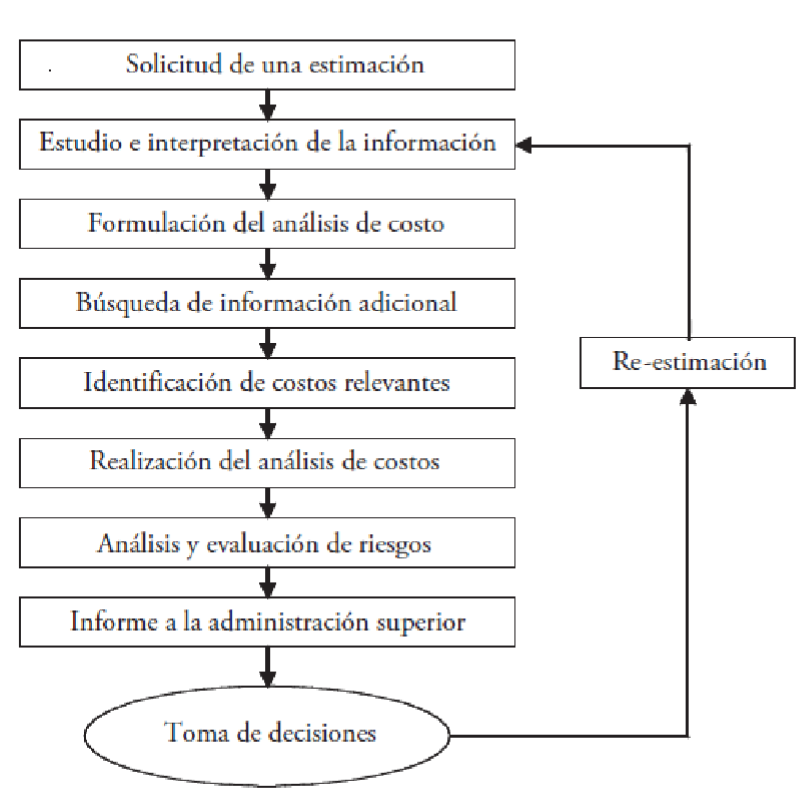
\includegraphics[width=\textwidth]{FOTOS/est_costos.png} % Reemplaza "imagen1.jpg" por el nombre de tu archivo
        \caption{Proceso de estimación de costos}
        \label{fig:imagen1}
    \end{subfigure}
    \hfill
    \begin{subfigure}[b]{0.45\textwidth}
        \centering
        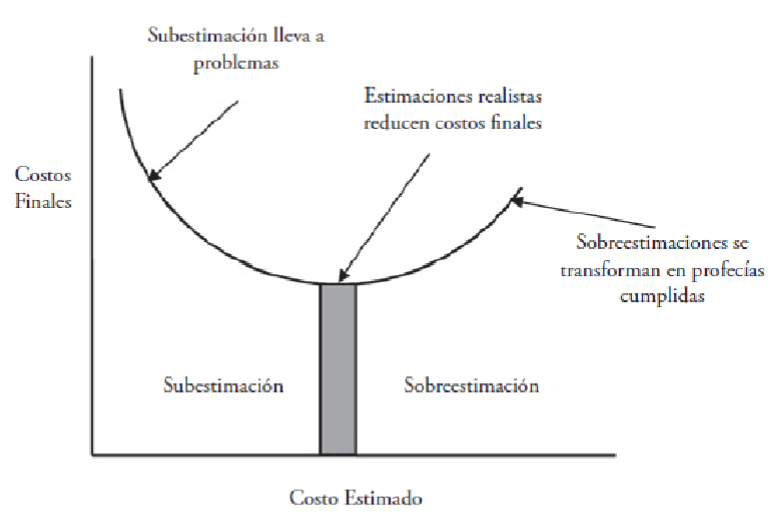
\includegraphics[width=\textwidth]{FOTOS/sub_costo.png} % Reemplaza "imagen2.jpg" por el nombre de tu archivo
        \caption{Importancia de la estimación}
        \label{fig:imagen2}
    \end{subfigure}
    \label{fig:imagenes_juntas}
\end{figure}

\subsubsection{Métodos para la estimación}

\begin{itemize}
    \item Paramétrica: Se basa en relaciones empíricas entre costos y parámetros de desempeño (tamaño, calidad, complejidad), considerando el método de construcción. Esto se conoce como CER (Cost Estimating Relationship).
    \item Factores: Aplica un factor a un ítem clave de costo para estimar otros ítems necesarios, basado en datos históricos.
    \item Modelo de costos: Utiliza un modelo estándar del proyecto que, procesando datos de costo, estima el costo total.
    \item Probabilística: Similar al PERT, incorpora riesgo mediante estimaciones múltiples (optimista, probable, pesimista) y evalúa la incertidumbre proporcional a la varianza.
\end{itemize}

\subsection{Estudio detallado de un presupuesto}

Un presupuesto total de una obra, o presupuesto de venta, es la estimación total que el ejecutor cobra al mandante. Incluye:

\begin{itemize}
    \item Presupuesto de diseño: Costo del diseño del proyecto, abarcando arquitectura, cálculo, instalaciones, etc.
    \item Costos directos: Estimación del costo de materiales, mano de obra y equipos directamente relacionados con actividades específicas.
    \item Gastos generales: Costos directos no imputables a una actividad específica, prorrateados en diferentes partidas (ej. salarios administrativos, consumibles).
    \item Gastos generales indirectos: 
    \begin{itemize}
        \item Costo financiero: Recursos necesarios para ejecutar las obras mientras se reciben los pagos o ingresos esperados.
        \begin{itemize}
            \item Garantías: Costos de las boletas de garantía requeridas en los contratos (ej. garantía de seriedad de la propuesta, buena ejecución).
            \item Gastos generales de oficina central: Contribución de la obra a la administración central, necesarios incluso sin obras (ej. sueldo gerente, oficinas, teléfonos).
        \end{itemize}
        \item Imprevistos: Riesgo de gastos no controlables. Disminuyen con mayor seguridad en precios y cantidades.
        \item Utilidad: Ganancia estimada, generalmente calculada como porcentaje del presupuesto del proyecto, dependiendo de rentabilidad, complejidad y riesgo.
        \item Impuestos: En Chile, las obras de construcción están sujetas al IVA. Las viviendas para compradores finales tienen un crédito del 65\%, reduciendo el IVA efectivo al 6,65\% (cuando el IVA es 19\%). Desde 2008, esta franquicia se limita a viviendas de hasta 3.000 UF y desaparece para aquellas de 4.500 UF.
    \end{itemize}
\end{itemize}

\subsubsection{Etapas para el estudio de un presupuesto}

\begin{enumerate}
    \item \textbf{Calendario de licitación}: Configuración de fechas clave para el análisis de precios, recepción de cotizaciones y revisión de ofertas.
    \item \textbf{Método constructivo}: Definición del método de construcción que determina el costo.
    \item \textbf{Estrategia presupuestaria}: Consideración de carga de trabajo, competidores, y tipo de proyecto.
    \item \textbf{Estudio de bases de licitación}: Análisis exhaustivo de plazos y condiciones impuestas por el mandante.
    \item \textbf{Cotizaciones}: Preparación de listas y solicitud de cotizaciones con especificaciones claras.
    \item \textbf{Subcontratos y cubicaciones}: Definición de prioridades en cubicaciones y análisis de contratos por precio unitario.
    \item \textbf{Estimación preliminar}: Realización de una estimación general del monto total.
    \item \textbf{Visita al terreno}: Evaluación in situ de las condiciones para la ejecución del proyecto.
    \item \textbf{Programación tentativa}: Elaboración de programas preliminares para optimizar recursos.
    \item \textbf{Revisión de precios locales}: Actualización de precios de mano de obra y maquinaria según condiciones locales.
    \item \textbf{Análisis detallado}: Estudio separado de costos directos, indirectos, gastos generales e imprevistos.
    \item \textbf{Revisión final}: Ajuste y verificación del presupuesto antes de la presentación de la oferta.
\end{enumerate}

\subsubsection{Estudio de costo directo}

Una vez aceptado el presupuesto, la omisión de algún ítem es una pérdida para el contratista. Las partidas deben ser medibles, presupuestables y controlables para cuantificar avances y comparar el progreso real con lo programado. Es recomendable identificar cada partida con un código y descripción, siguiendo la norma NCh 1156 Of. 99.

El segundo paso es definir la unidad de medida de cada partida, basada en las especificaciones técnicas o en la norma NCh 353 Of 2000. El tercer paso es cubicar las partidas, calculando las cantidades necesarias en volumen, área o longitud según la norma NCh 353 Of 2000.

El cuarto paso es estimar el costo de la partida mediante un análisis de precios unitarios. El costo directo o precio unitario (P.U.) debe incluir todos los costos directos necesarios para ejecutar el trabajo y ser compatible con las bases de medición. Se compone de cuatro elementos clave:

\begin{itemize}
    \item \textbf{Mano de obra}: Costo del personal involucrado, según especialidad y productividad.
    \item \textbf{Materiales}: Costo de los materiales en obra, basado en la cubicación y especificaciones técnicas.
    \item \textbf{Maquinaria y equipos}: Costo de equipos y herramientas, determinado por la planificación y estrategia de la obra.
    \item \textbf{Otros costos}: Herramientas y elementos menores que se requieren para una faena.
\end{itemize}

\subsubsection{Costo base de la mano de obra}

El costo de la mano de obra varía según las especialidades involucradas en un proyecto (profesionales, técnicos, maestros, ayudantes, administrativos, etc.). Factores que afectan su variabilidad incluyen:

\begin{itemize}
    \item Exigencia de habilidades especiales.
    \item Exigencia de conocimientos específicos.
    \item Exigencia de condiciones físicas especiales.
    \item Demanda de mano de obra en el mercado.
\end{itemize}

Para evaluar correctamente el costo, es importante estimar el rendimiento del trabajador, considerando que su tiempo en obra se divide en:

\begin{itemize}
    \item \textbf{Trabajo productivo} (60\%): Aporta directamente a la producción (e.g., colocación de moldajes).
    \item \textbf{Trabajo contributorio} (25\%): Actividades de apoyo necesarias (e.g., limpieza de superficies).
    \item \textbf{Trabajo no contributorio} (15\%): Acciones no productivas (e.g., espera por recursos).
\end{itemize}

Definiciones importantes:

\begin{itemize}
    \item \textbf{Remuneración (R)}: Pagos en dinero o en especies que recibe el trabajador por contrato.
    \item \textbf{Remuneración imponible (Ri)}: Parte de la remuneración usada para calcular imposiciones.
    \item \textbf{Sueldo}: Salario fijo determinado por contrato, pagado diaria o mensualmente. El sueldo líquido es el monto después de impuestos.
    \item \textbf{Pago por semana corrida}: Derecho a remuneración por domingos y festivos, condicionado a la asistencia semanal.
    \item \textbf{Gratificación}: Recompensa basada en utilidades de la empresa o un monto fijo anual de 4,75 salarios mínimos.
    \item \textbf{Feriado legal}: Derecho a 15 días hábiles de vacaciones anuales con remuneración íntegra.
    \item \textbf{Imposiciones}: Porcentajes sobre Ri destinados a fondos de pensiones y salud.
\end{itemize}

\noindent Los siguientes pagos no constituyen remuneración:
\begin{itemize}
    \item Asignación de movilización.
    \item Asignación por colación.
    \item Asignación por pérdidas de caja.
    \item Asignación por desgaste de herramientas.
    \item Viáticos (traslados, alojamiento y comidas con rendición).
    \item Prestaciones familiares por ley.
    \item Devolución de gastos por trabajo.
\end{itemize}

\textbf{El Trato}

Consiste en un convenio entre el empleador y el trabajador, o entre la empresa constructora y el subcontratista, según sea el caso, mediante el cual se fija un monto de dinero por realizar una faena específica en un plazo determinado.

\begin{equation}
    \text{TRATO} = (\text{Sueldo Base}) + (\text{Cantidad efectivamente realizada} \times \text{Precio de la unidad})
\end{equation}

Se utiliza para pagar faenas que son repetitivas o de un volumen importante en la construcción.

Para los convenios directos entre empleador y trabajador se utiliza directamente la fórmula anterior, en cambio en el caso de los subcontratos sólo se utiliza el segundo término de la ecuación.

La principal ventaja de utilizar el trato es obtener una mayor productividad en la obra.

La principal desventaja que este sistema de pago presenta, es que en ciertas ocasiones los trabajadores o los subcontratistas se despreocupan de la calidad requerida

\textbf{Componentes del costo de la mano de obra}

El costo de un trabajador incluye un costo fijo, un costo variable, un costo adicional por leyes sociales y costos asociados a gastos generales de faena.

\begin{itemize}
    \item \textbf{Costo fijo}: Incluye la remuneración del trabajador, considerando vacaciones, derecho a semana corrida e imposiciones. También puede incluir gratificaciones pagadas mensualmente. En construcción, considerando una jornada de lunes a sábado, se trabajan aproximadamente:
    \begin{equation}
        \text{Horas anuales trabajadas} = 300 \, \text{días} \times 8 \, \text{horas/día} = 2400 \, \text{horas}
    \end{equation}
    Además, debe sumarse el pago de los días domingos, en caso de que el contrato sea por día, según el Código del Trabajo. El ingreso anual por domingos es:
    \begin{equation}
    \text{Ingreso por domingos} = 53 \, \text{domingos} \times 8 \, \text{horas} \times 1.100 = 466.400 \, \text{pesos}
    \end{equation}
    \item \textbf{Costo variable}: 
    \begin{itemize}
        \item \textbf{Costos variables mensuales}:
        \begin{itemize}
            \item \textbf{Sobretiempo}: Recargo del 50\% en días hábiles y 100\% en domingos y festivos.
            \item \textbf{Trato}: Mayor costo dependiendo del coeficiente de trato.
            \item \textbf{Participaciones de producción}: Según se considere en la obra.
        \end{itemize}
        
        \item \textbf{Costo variable anual}:
        \begin{itemize}
            \item Gratificaciones y participaciones de producción anual, o 4,75 ingresos mínimos.
        \end{itemize}
    \end{itemize}
    \item \textbf{Costo adicional CAT}:
    \begin{itemize}
        \item \textbf{Seguro de accidentes}: Un 3\% sobre el total ganado.
        \item \textbf{Seguro de desempleo}: Contribuciones del 0,6\% del trabajador y 2,4\% del empleador.
        \item \textbf{Aporte patronal}: Corporación Habitacional (0,9\%) y Servicio Médico (2,1\%).
    \end{itemize}
    \item \textbf{Asignaciones}:
    \begin{itemize}
        \item \textbf{Asignación de alimentación}:
        \begin{equation}
        \text{Asignación de alimentación} = 300 \, \text{días} \times 200 = 60.000 \, \text{pesos}
        \end{equation}
        \begin{equation}
        \text{Asignación de alimentación (\%)} = \frac{60.000}{3.106.400} = 1,9\%
        \end{equation}
        
        \item \textbf{Asignación de movilización}:
        \begin{equation}
        \text{Asignación de movilización} = 300 \, \text{días} \times 600 = 180.000 \, \text{pesos}
        \end{equation}
        \begin{equation}
        \text{Asignación de movilización (\%)} = \frac{180.000}{3.106.400} = 5,8\%
        \end{equation}
        
        \item \textbf{Asignación por desgaste de herramientas}:
        \begin{equation}
        \text{Asignación por herramientas} = 300 \, \text{días} \times 400 \times 0,4 = 48.000 \, \text{pesos}
        \end{equation}
        \begin{equation}
        \text{Asignación por herramientas (\%)} = \frac{48.000}{3.106.400} = 1,5\%
        \end{equation}
    \end{itemize}
    \item \textbf{Indemnizaciones}: Costos en los que se incurre al despedir a un trabajador sin causa de caducidad de contrato según la ley. Los casos específicos son:
    \begin{itemize}
        \item \textbf{Desahucio}: Pago de un mes de sueldo al trabajador despedido sin previo aviso de al menos un mes. En obras transitorias como la construcción, este pago no se aplica.
        
        \item \textbf{Indemnización por años de servicio}: Pago de un mes de sueldo por cada año trabajado, con un tope máximo según la ley. En la construcción, generalmente no se paga en obras transitorias.
        
        \item \textbf{Pago proporcional por vacaciones}: Compensación al trabajador despedido antes de tomar sus vacaciones. Se le paga una cantidad proporcional a los días que le corresponderían según el tiempo trabajado.
    
        \item \textbf{Feriado anual (vacaciones)}:
        \begin{equation}
        \text{Feriado anual} = 21 \, \text{días} \times 8 \, \text{horas} \times 1.100 = 184.800 \, \text{pesos}
        \end{equation}
        \begin{equation}
        \text{Feriado anual (\%)} = \frac{184.800}{3.106.400} = 5,9\%
        \end{equation}
        
        \item \textbf{Causas climáticas}:
        \begin{equation}
        \text{Clima} = 10 \, \text{días} \times 8 \, \text{horas} \times 1.100 = 123.200 \, \text{pesos}
        \end{equation}
        
        \item \textbf{Días festivos}:
        \begin{equation}
        \text{Festivos} = 14 \, \text{días} \times 8 \, \text{horas} \times 1.100 = 88.000 \, \text{pesos}
        \end{equation}
        \begin{equation}
        \text{Festivos (\%)} = \frac{88.000}{3.106.400} = 4,0\%
        \end{equation}
        
        \item \textbf{Aguinaldos}:
        \begin{equation}
        \text{Aguinaldos} = 2 \times 25.000 = 50.000 \, \text{pesos}
        \end{equation}
        \begin{equation}
        \text{Aguinaldos (\%)} = \frac{50.000}{3.106.400} = 1,6\%
        \end{equation}
    \end{itemize}
\end{itemize}

\begin{figure}[H]
    \centering
    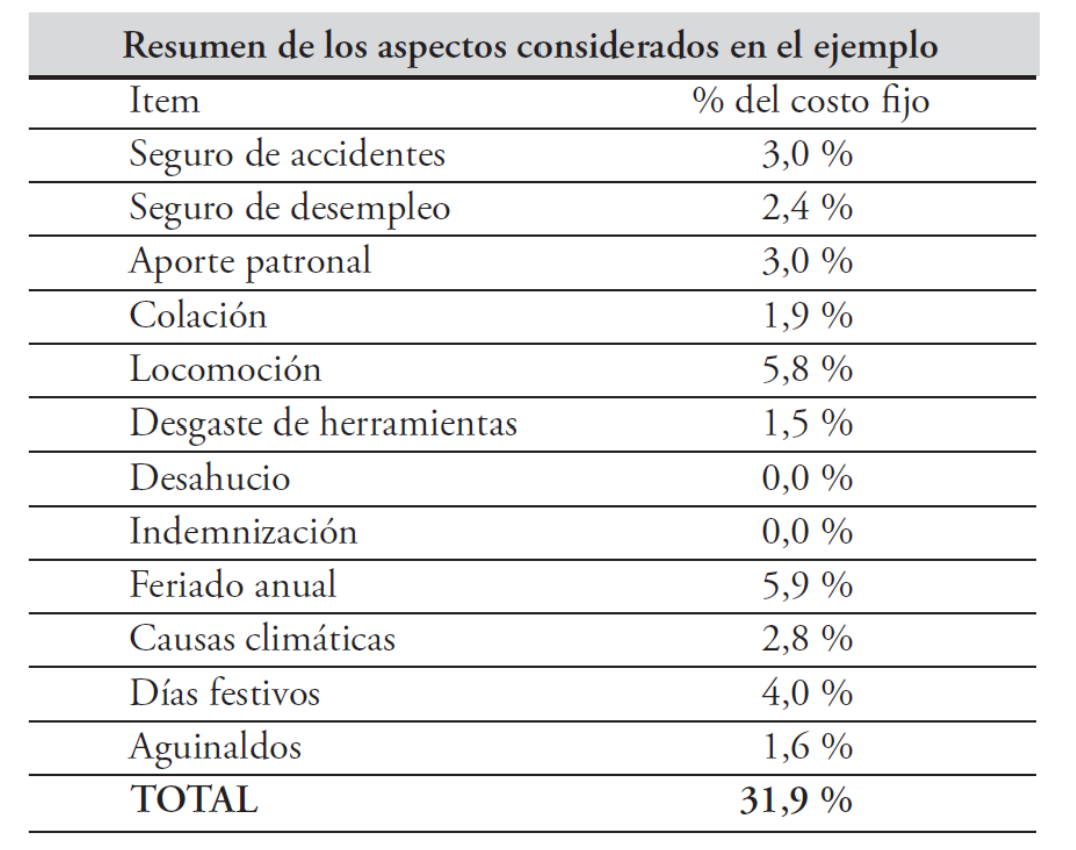
\includegraphics[width=0.7\textwidth]{FOTOS/indem.png}
    \label{fig:costo_mo}
\end{figure}

\subsubsection{Costo base de los materiales}

El costo de los materiales se basa en una cotización adecuada de los materiales a utilizar en la obra, diferenciada por tipo y considerando al proveedor más conveniente. El precio debe ser puesto en obra y puede verse afectado por varios factores:
\begin{itemize}
    \item \textbf{Formas de pago}
    \item \textbf{Volúmenes de compra}
    \item \textbf{Calidad de los materiales}
    \item \textbf{Ofertas del momento}
    \item \textbf{Otros factores}
\end{itemize}

Al analizar el costo de materiales, es recomendable incluir posibles pérdidas debido a:

\begin{itemize}
    \item Robos
    \item Mala utilización
    \item Mal almacenamiento
    \item Mal transporte
    \item Otras pérdidas significativas
\end{itemize}

\subsubsection{Costo base de los equipos}

En este rubro se incluyen herramientas (martillos, palas, carretillas, etc.), útiles (escaleras, andamios, etc.) y maquinarias (grúas, vibradores, etc.). En muchas empresas, el costo de herramientas y útiles se carga a gastos generales, mientras que para las maquinarias existen tres opciones:

\begin{itemize}
    \item \textbf{Equipos arrendados}: Se considera una tasa de arriendo, teniendo en cuenta qué costos están incluidos. Si ciertos costos como operador, mantención o accesorios no están incluidos, deben agregarse para estimar el costo real de operación.
    
    \item \textbf{Equipos con leasing}: Utilizan un instrumento financiero que implica un arriendo con compromiso de compra. El costo mensual es generalmente superior al de un arriendo tradicional, pero ofrece beneficios tributarios. Al final del período de leasing, se puede adquirir el equipo con una cuota adicional.
    
    \item \textbf{Equipos propios}: Requiere determinar los costos de depreciación, posesión y operación mediante algún método específico, que se desarrollará en el capítulo correspondiente.
\end{itemize}

\subsection{Precio unitario}

Conocidos los costos de los componentes principales de cada partida, se debe justificar su precio unitario. Para calcular estos precios se determina el costo total de la partida y se divide por la cantidad de unidades respectivas, considerando economías o deseconomías por volumen de obra.

Por ejemplo, el costo unitario de 100.000 m³ de hormigón es menor que el de 10 m³ debido a variaciones en precios de insumos y prorrateo de equipos. Otra opción es estimar el precio unitario de cada partida independientemente de la cubicación, considerando sólo materiales, equipos y personal necesarios para la unidad (e.g., m², ml, gl, UN). También es posible una combinación de ambos métodos para diferentes partes de la obra.

\begin{figure}[H]
    \centering
    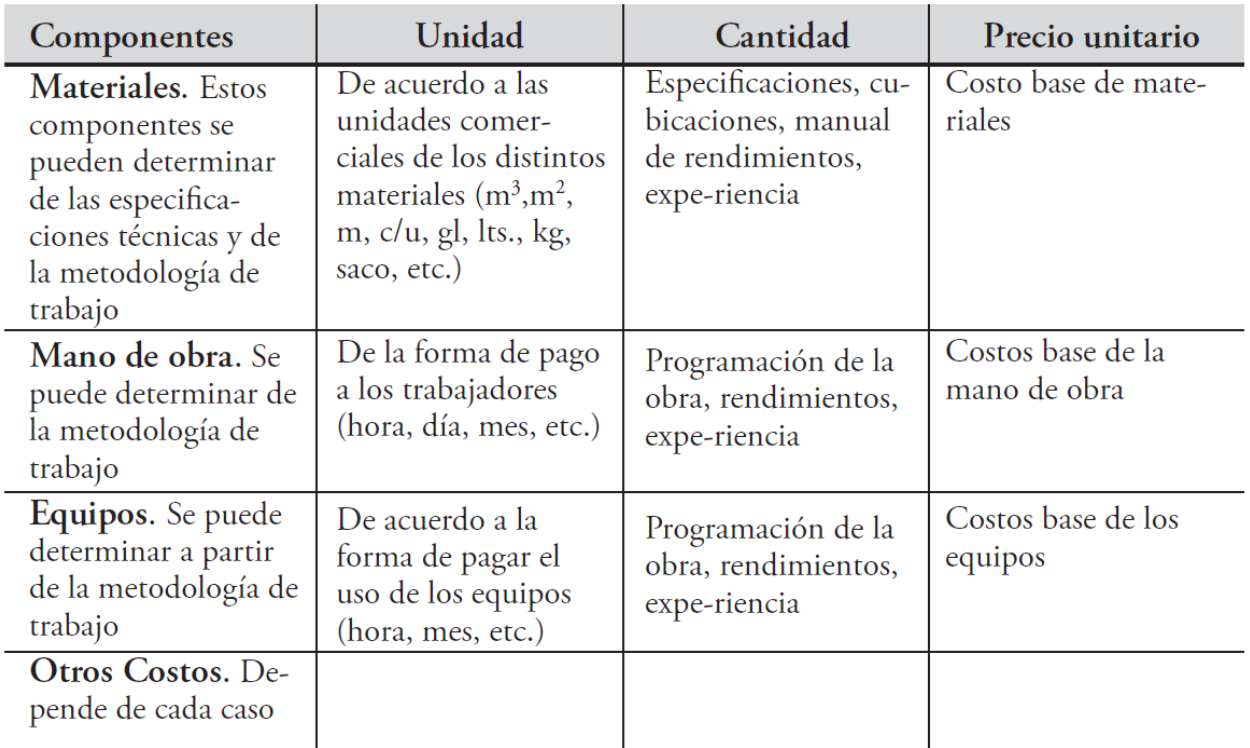
\includegraphics[width=0.7\textwidth]{FOTOS/pu.png}
    \label{fig:precio_unitario}
\end{figure}

\subsection{Gastos}

\subsubsection{Gastos generales}

El cálculo de los gastos generales se divide en tres grupos principales:

\begin{itemize}
    \item \textbf{Personal}: Incluye gastos de personal no directamente involucrado en la ejecución de la obra.
    \begin{itemize}
        \item \textbf{Personal administrativo y de apoyo}: Profesionales, administrativos, laboratoristas, supervisores, jefes de turno, mecánicos, eléctricos, etc.
        \item \textbf{Asesores}: Auditores, calculistas, abogados, medio ambiente, seguridad.
        \item \textbf{Entretenciones}: Fiestas de los tijerales, club deportivo.
    \end{itemize}
    
    \item \textbf{Instalaciones}: Incluye todo lo relacionado con la operación de la obra.
    \begin{itemize}
        \item \textbf{Instalaciones de faena}: Oficinas, servicios higiénicos, talleres, bodegas, plantas, galpones, laboratorios.
        \item \textbf{Movilización}: Vehículos para personal, ambulancias, camionetas.
        \item \textbf{Viajes y visitas}: Costos de visitas y viajes de la empresa.
        \item \textbf{Gastos de oficina de obra}: Papelería, fotocopias, planos, correspondencia.
        \item \textbf{Gastos de servicios}: Agua, luz, telefonía, internet.
        \item \textbf{Policlínico}: Materiales médicos.
        \item \textbf{Seguridad e higiene}: Elementos de seguridad, señalización.
    \end{itemize}
    
    \item \textbf{Equipamiento}: Vehículos, fletes, equipos de laboratorio, computación y comunicaciones. Si no están en el precio unitario, se deben incluir aquí.
    \begin{itemize}
        \item \textbf{Fletes}: Ida y retorno de equipos, materiales y mudanzas de personal.
        \item \textbf{Control de calidad}: Laboratorio externo.
        \item \textbf{Topografía}: Arriendo y mantenimiento de equipos, estacas, puntos de referencia.
        \item \textbf{Comunicaciones}: Radio, teléfono, internet.
        \item \textbf{Despachos}: Correspondencia y encomiendas.
    \end{itemize}
\end{itemize}

\subsubsection{Gastos generales indirectos}

Los gastos generales indirectos son aquellos que se generan por la realización del proyecto, pero no directamente por su construcción, como la oficina central, costos financieros, varios e imprevistos.

\begin{itemize}
    \item \textbf{Oficina Central}: El costo de la oficina central de la empresa debe distribuirse entre todas las obras activas. El cálculo se realiza estimando un porcentaje del costo directo, o bien, se pueden considerar por separado los siguientes costos:
    \begin{itemize}
        \item \textbf{Gastos de oficina general}: Contabilidad, administración, etc.
        \item \textbf{Gastos de representación}: Publicidad, atención a personalidades, eventos.
    \end{itemize}
    
    \item \textbf{Costo Financiero}: Se calcula a partir del flujo de caja neto del proyecto, estimando la diferencia entre los gastos programados y los ingresos esperados. La estimación se basa en el programa mensual de inversiones y el flujo mensual de gastos generales. La tasa de interés utilizada depende del banco o indicador financiero de referencia.
    
    \item \textbf{Costos Indirectos Varios}: Gastos asociados a efectos del proyecto, asesorías y aspectos legales. Algunos ejemplos son:
    \begin{itemize}
        \item \textbf{Gastos de propuesta}: Costos de estudio, viajes, etc.
        \item \textbf{Garantías}: Boletas de seriedad, garantía de cumplimiento y correcta ejecución.
        \item \textbf{Costos de notaría}: Escrituras de contrato, protocolizaciones.
        \item \textbf{Derechos y permisos}: Permisos municipales, exploración de canteras, permisos de agua.
        \item \textbf{Seguros}: Responsabilidad civil, vehículos, vida de empleados, daños a terceros, incendio, equipos. Existe un seguro a todo riesgo de construcción que cubre al personal, equipos y obra desde el inicio hasta la finalización del proyecto.
    \end{itemize}
\end{itemize}

\subsection{Presentación de un presupuesto}

La presentación de presupuestos es similar para cada tipo de contrato, pero la interpretación varía según el tipo:

\begin{itemize}
    \item \textbf{Administración delegada}: El presupuesto es una buena estimación del costo, ya que el dueño cubrirá todos los gastos incurridos por el contratista. Es esencial definir los honorarios del contratista.
    
    \item \textbf{Contratos a serie de precios unitarios}: Lo importante son las partidas y sus precios unitarios, ya que las cantidades son estimaciones. El mandante pagará al contratista por las cantidades efectivamente ejecutadas a los precios unitarios acordados.
    
    \item \textbf{Contratos de suma alzada}: La presentación del presupuesto es referencial, ya que el dueño pagará el monto total acordado independientemente de las estimaciones.
\end{itemize}

\begin{figure}[H]
    \centering
    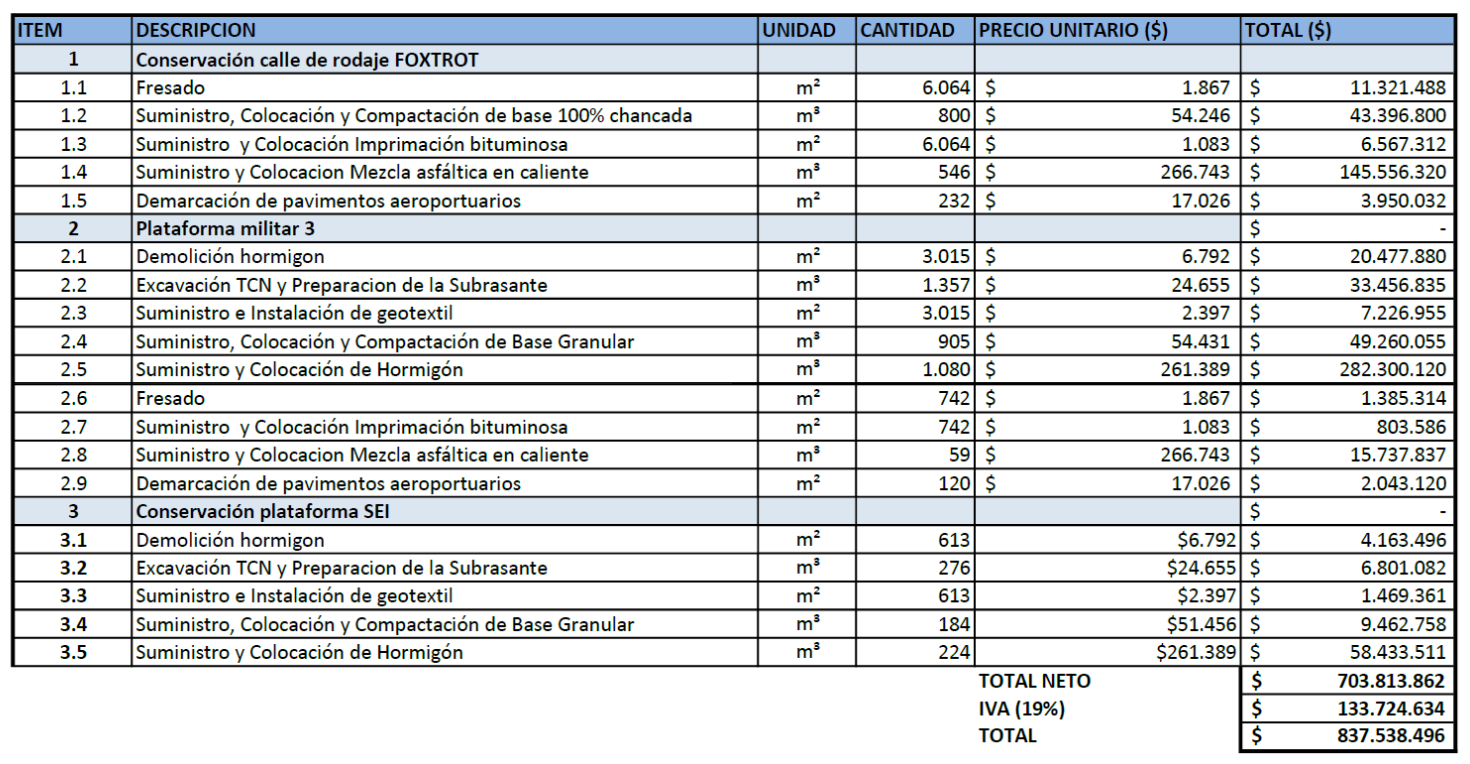
\includegraphics[width=0.8\textwidth]{FOTOS/ej_pu.png}
    \label{fig:presupuesto}
\end{figure}

Para la presentación del presupuesto u oferta final, la empresa constructora debe distribuir todos los gastos distintos a los costos directos en las partidas consideradas ítems de pago. Existen varias opciones para hacerlo, como la distribución porcentual. Además, la oferta final puede variar según la estrategia adoptada para la propuesta, ajustándose según el interés del contratista en la obra o la carga de trabajo existente.

El uso de tecnología computacional facilita el estudio de presupuestos, acelerando el proceso. Sin embargo, la responsabilidad final recae en quien usa el programa. Las empresas pueden diseñar sus propios programas o adquirir alguno disponible en el mercado. En Chile, algunos programas comunes para el estudio de presupuestos son: Notrasnoches (plataforma ONDAC), Presto y Unysoft.

\subsubsection{Reajuste de presupuesto}

Las obras de construcción suelen tener períodos de ejecución prolongados, lo que hace necesario considerar reajustes de precios para actualizar los montos. Estos reajustes se aplican en los pagos parciales o al término de la obra. Las formas de considerar los reajustes incluyen:

\begin{itemize}
    \item \textbf{Índice Reajustable}: Confeccionar el presupuesto sobre la base de un índice que pueda ser reajustado, como la UF.
    
    \item \textbf{Polinomios de Reajustes}: Utilizar polinomios que combinan diferentes índices en proporciones adecuadas para reflejar la variación real del costo de la obra.
    
    \item Ejemplo de Reajuste:
    \begin{align}
    \text{Reajuste} &= 0.20 \times \text{(variación del costo de la mano de obra)} \nonumber \\
    &\quad + 0.40 \times \text{(variación del precio de los materiales)} \nonumber \\
    &\quad + 0.10 \times \text{(variación del dólar)} \nonumber \\
    &\quad + 0.30 \times \text{(variación de la unidad de fomento)}
    \end{align}  
\end{itemize}

En contratos con cláusulas de reajuste de precios, es recomendable considerar la posible diferencia entre el índice contractual de reajuste y la variación real del costo. Si se prevé una diferencia significativa, se sugiere ajustar el presupuesto en consecuencia. Este aspecto es especialmente importante en proyectos sin reajustes.

El MOP ofrece tres opciones para reajustes: sin reajustes, con reajuste de IPC, y la opción polinómica.

Si el IPC es reemplazado por otro índice determinado por el INE o la autoridad competente, el reajuste se calculará con base en el nuevo índice. El pago del reajuste se realizará junto con el estado de pago de obra correspondiente.

Cuando se realicen pagos de reajuste en los contratos, su valor se ajustará automáticamente, ya sea aumentando o disminuyendo, sin esperar la resolución final. En caso de discrepancias en estas resoluciones, las retenciones y garantías del contrato cubrirán posibles excesos pagados. Los precios unitarios acordados en el contrato se mantendrán vigentes para otros efectos, excepto para temas de presupuesto y pago.

\subsection{Sistemas de Pago}

En Chile, la modalidad más común en obras es la de **Estados de Pago (EP)**, que refleja el avance físico de la obra en términos monetarios. Considera elementos como avance físico, retenciones, descuentos y devoluciones. El proceso de pago incluye:

\begin{itemize}
    \item \textbf{Detalle de Estado de Pago}:
    \begin{itemize}
        \item Antecedentes de obra
        \item Número correlativo y período
        \item Partidas contempladas
        \item Monto contratado (unidad, cantidad, P.U.)
        \item Obra realizada hasta la fecha (unidad, cantidad, P.U., total)
        \item Valor realizado hasta el estado de pago anterior (total)
        \item Valor del presente estado de pago (diferencia entre el actual y el anterior EP)
    \end{itemize}
    
    \item \textbf{Carátula del Estado de Pago}:
    \begin{itemize}
        \item Antecedentes de obra
        \item Número de estado de pago y período que abarca
        \item Valor realizado a la fecha
        \item Valor realizado hasta el estado de pago anterior
        \item Retenciones
        \item Devoluciones
        \item Descuentos
        \item Líquido a pagar
    \end{itemize}
    
    \item \textbf{Factura}
\end{itemize}

El estado de pago debe ser revisado y aprobado por la inspección antes de ser pagado por el dueño. Los pagos pueden realizarse en diferentes períodos de tiempo, de acuerdo con las condiciones estipuladas en el contrato.

\begin{figure}[H]
    \centering
    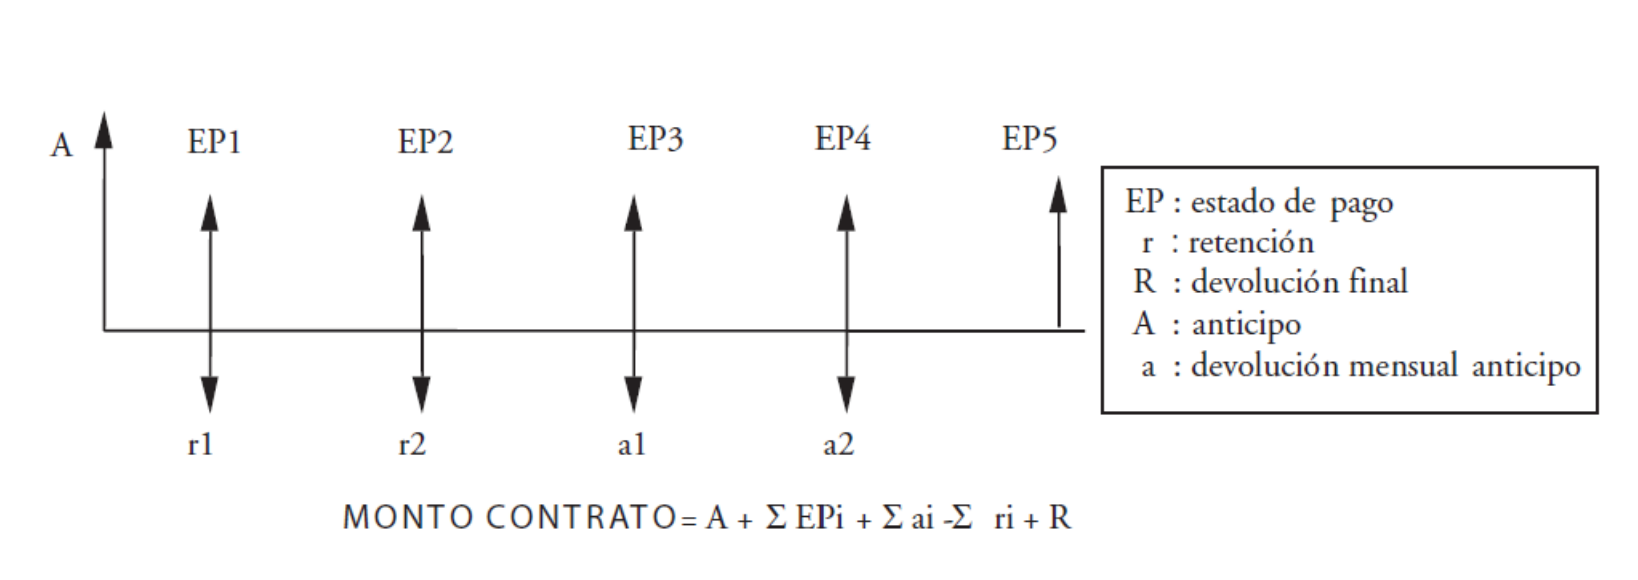
\includegraphics[width=0.8\textwidth]{FOTOS/sist_pag.png}
    \label{fig:estado_pago}
\end{figure}






\part{Capítulo 6}
\section{Clasificación de estructuras}
\begin{itemize}
    \item Clase A: Edificios de acero con losas de homigón armado o entrepisos de acero
    \item Clase B: Edificios de hormigón con losas de hormigón o estructuras mixtas de hormigón y acero
    \item Clase C: Edificios de albañilería de ladrillo confinado entre cadenas y pilares de hormigón armado
    \item Clase D: Edificios de albañileria de bloques o piedras confinado entre cadenas y pilares de hormigón armado
    \item Clase E: Edificios de estructuras de madera, con entrepisos de madera
    \item Clase F: Edificios de estructuras de adobe, con entrepisos de madera
    \item Clase G: Edificios de estructuras prefabricadas de madera, acero u hormigón
    \item Clase H: Edificios de estructuras prefabricadas de madera
    \item Clase I: Edificios de estructuras prefabricadas o paneles de hormigón liviano, fibrocemento o poliestireno expandido
\end{itemize}

\section{Componenetes de una edificación}
\begin{itemize}
    \item Infraestructura o Fundación
    \item Supraestructura o Cuerpo
    \item Techumbre
    \item Terminaciones
    \item Instalaciones
\end{itemize}

\subsection{Urbanización}
\begin{itemize}
    \item Trazados viales y urbanos
    \item Áreas verdes y equipamientos
    \item Iluminación y ventilación
    \item Dotación de servicios sanitarios, energéticos y de comunicación
\end{itemize}
\subsection{Instalación de Faenas}
Instalaciónes provisorias de apoyo a la construcción de la obra
\begin{itemize}
    \item Cierro provisorio
    \item Portería e ingresos
    \item Instalaciones Administrativas
    \item Instalaciones de Personal
    \item servicios
    \item Servicios Básicos
    \item Caminos de acceso y de circulación
\end{itemize}
\subsection{Topografía}
Es la medición y representación de la superficie terrestre
\begin{itemize}
    \item Mapas: (1:250.000 a 1:2.500.000)
    \item Cartas: (1:25.000 a 1:100.000)
    \item Planos: (1:10 a 1:1.000)
    \item Se usa coordenadas UTM
    \item levantamiento topográfico
    \begin{itemize}
        \item Obtención de datos
        \item Procesamiento de datos
        \item Confección de planos
    \end{itemize}
    \item Replanteo para una verificación y control
\end{itemize}

\part{Capitulo 7}

\section{Tipos de Equipos}

\begin{itemize}
    \item Movimiento de Tierras
    \begin{itemize}
        \item Excavadoras (orugas con pala frontal)
        \item Buldozer
        \item Camion Tolva
        \item Retro Excavadora (Pala delantera y brazo atras)
        \item Mononiveladora (Niveladora de caminos)
        \item Motoniveladora (Igual pero con motor)
        \item Cargador Frontal (Pala frontal grande con articulacion en vehiculo y no en las ruedas)
        \item Mototrailla o Trailla (Permite ditribuir tierra)
    \end{itemize}
    \item Compactacion o Nivelacion
    \begin{itemize}
        \item Placa Compactadora (Se usa manualmente)
        \item Rodillo compactador liso (Hay de distintos tamaños)
        \item Rodillo compactador pata de cabra (Se usa para compactar mas profundamente)
        \item Rodillo compactador neumatico (Se usa para compactar asfalto, el que tiene muchas ruedas)
    \end{itemize}
    \item Produccion de Hormigon, existen distintos tipos de maquinas o instalaciones
\end{itemize}

\textbf{Criterios de Seleccion:} Se debe considerar el costo total, lo que comprende la inversion original mas el costo de operacion, costo de reparacion y mantencion del equipo. La suma de todo esto se define como \textbf{INVERSION TOTAL DE UN EQUIPO}

\section{Productividad de Equipos}

De este modo, se busca la productividad optima \textbf{Qp} la cual se basa en la operacion continua de la maquinaria por hora. Se define la productividad normal \textbf{Qv} como Qv incorporando el factor humano (0.85). Ademas si se agrega el factor de direccion del trabajo (fp), se optiene la productividad real \textbf{Qr}

\begin{equation}
    Qr = fp \cdot Qn = fp \cdot fw \cdot Qp = fa \cdot Qp
\end{equation}

\newpage
\section{Costos de Equipos}

Hay que tomar en consideracion costos como depreciacion e inversion inicial:

\begin{figure}[H]
    \centering
    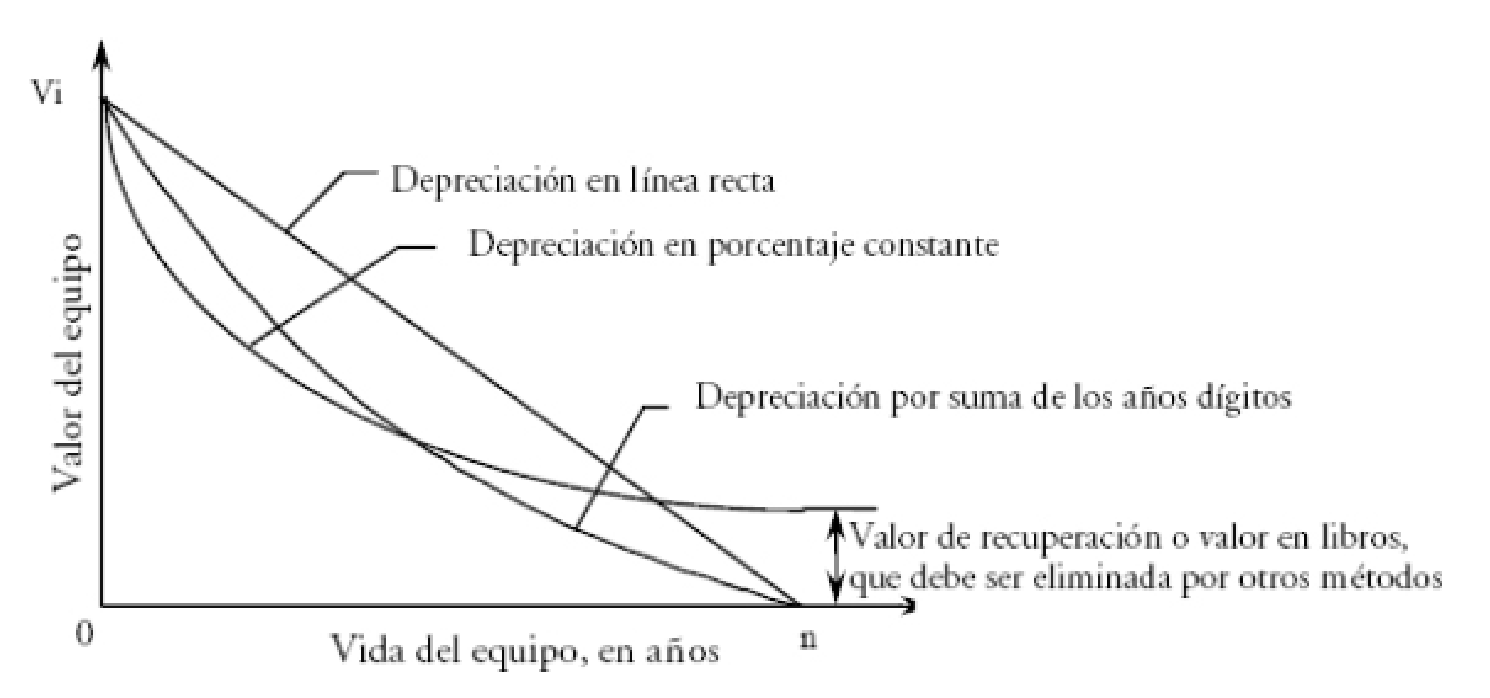
\includegraphics[width=0.8\linewidth]{FOTOS/costo_equipo.png}
    \caption{Costos de Equipos}
    \label{fig:costos}
\end{figure}

\begin{itemize}
    \item Costos de inversion
    \begin{itemize}
        \item Compra 
        \item Internacion
        \item Flete
        \item Seguro de traslado
        \item Intereses
        \item Impuestos
        \item Seguro
        \item Almacenaiento
    \end{itemize}
    \item Costos de operacion
    \begin{itemize}
        \item Operador
        \item Combustible
        \item Lubricacion
        \item mantencion
        \item Reparaciones menores
        \item Neumaticos y Filtros
    \end{itemize}
\end{itemize}

\newpage
\section{Vida Equipo}

De esta forma, la vida de un equipo se define como:

\begin{figure}[H]
    \centering
    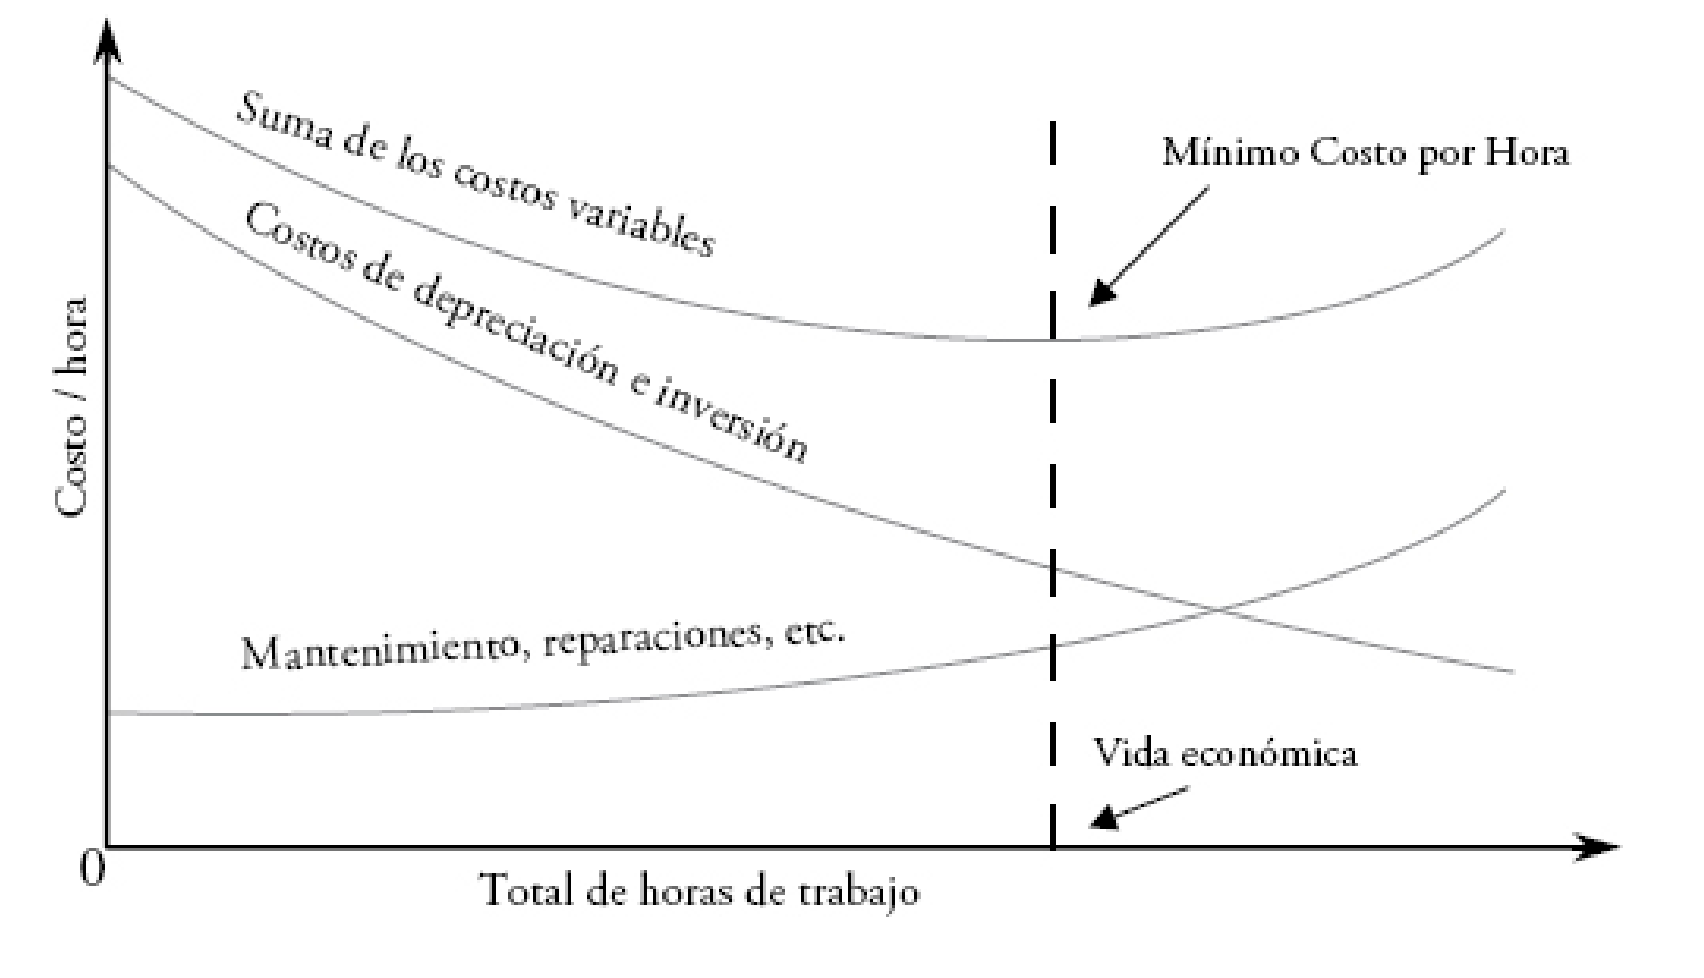
\includegraphics[width=0.8\linewidth]{FOTOS/vida_equipo.png}
    \caption{Vida de un Equipo}
    \label{fig:vida}
\end{figure}

\part*{Capítulo 8}

\section{Movimiento de tierra}
\begin{itemize}
    \item Desmalezar el terreno
    \item Remover estructuras y árboles existentes
    \item Nivelar el terreno
    \item Señalizar las obras y colocar protecciones
    \item Planificar la circulación de vehículos, maquinarias y personas
    \item Planificar el retiro de escombros
    \item Proteger estructuras y árboles existentes
    \item Determinar las técnicas a emplear para la evacuación de agua subterránea o de superficie
    \item Precauciones especiales con el medio ambiente
\end{itemize}

Antes de iniciar cualquier obra, es necesario replantear los planos en el terreno, marcando referencias que permitan verificar distancias, cotas y ángulos durante la excavación y construcción. Tras las excavaciones, se debe verificar nuevamente el replanteo. En grandes movimientos de tierra, se recomienda escarificar la capa superficial (10 a 20 cm) y almacenarla para reutilizarla. Esto evita la importación de material y ayuda a recuperar semillas y microorganismos locales, favoreciendo un equilibrio ambiental más rápido.

Una excavación puede hacerse empleando variadas técnicas, según las condiciones del proyecto y las restricciones específicas. Algunas son:
\begin{itemize}
    \item Tipo de proyecto de ingeniería.
    \item Tamaño y profundidad de la excavación.
    \item Tipo de terreno (roca o suelo, tipo de estratificación, etc.).
    \item Calidad del suelo (inclinación de taludes o protecciones).
    \item Estructuras contiguas.
    \item Restricciones de espacio.
    \item Equipo y maquinaria disponible.
    \item Presencia de agua subterránea o superficial.
    \item Condiciones ambientales.
\end{itemize}

En trabajos pequeños y en suelo blando, la tierra se puede excavar con palas y picota si se requiere. En excavaciones abiertas con volúmenes mayores de movimiento de tierra se debe considerar el empleo de equipos especializados, como:
\begin{itemize}
    \item Palas Mecánicas: cargadores frontales, retroexcavadoras, palas frontales.
    \item Dragas.
    \item Grúas con cucharón de almeja.
    \item Zanjadoras y otros.
\end{itemize}

\begin{itemize}
    \item \textbf{Excavación de zapata}: Excavación de dimensiones similares (largo, ancho y profundidad).
    \item \textbf{Excavación en zanja}: Excavación larga y angosta (ancho entre 0.5 m y 3.2 m) para fundaciones corridas o canalizaciones.
    \item \textbf{Excavaciones amplias}: Excavaciones de más de 3.2 m de ancho, usadas para subterráneos y grandes fundaciones.
    \item \textbf{Pozos}: Excavaciones profundas y de forma rectangular o circular, para captación de agua o prospección de suelos.
\end{itemize}

Una excavación abierta se puede diseñar de las siguientes formas:
\begin{itemize}
    \item \textbf{Taludes libres}: vertical, inclinado, escalonado.
    \item \textbf{Taludes protegidos}: apuntalados, entibados.
\end{itemize}

Los factores y condiciones especiales de la obra que lo condicionan son:
\begin{itemize}
    \item Tipo de terreno.
    \item Costo relativo entre ambas soluciones.
\end{itemize}

Los factores que condicionan la excavación son:
\begin{itemize}
    \item \textbf{Tiempo de apertura}: Si es prolongado, es recomendable proteger los taludes, especialmente en zonas sísmicas o con vibraciones.
    \item \textbf{Asentamientos permisibles} alrededor de la excavación.
    \item \textbf{Presencia de agua}.
\end{itemize}

\textbf{Excavaciones con talud libre}: Para excavaciones mayores a 1.2 m de profundidad, si el terreno es cohesivo y permite un talud vertical, se puede realizar sin entibación si se ha calculado la altura crítica de excavación (Hc). La ecuación para Hc es:

\[
Hc = 1.3 \frac{q_u}{\gamma}
\]

donde:
\begin{itemize}
    \item $qu$: resistencia al corte de una muestra de suelo, en kg/m².
    \item $\gamma$: densidad natural del terreno, en kg/m³.
\end{itemize}

Esta fórmula es válida si cualquier sobrecarga en el borde de la excavación está a una distancia mayor que la profundidad de la excavación (Hs).


\begin{figure}[h]
    \centering
    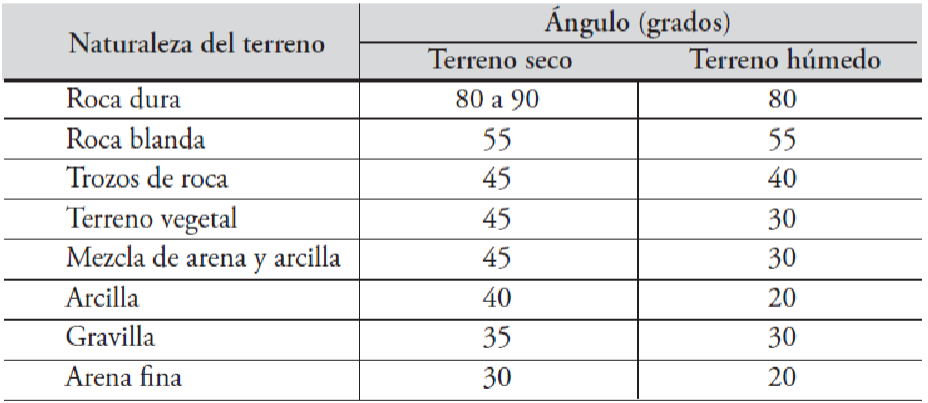
\includegraphics[width=0.8\textwidth]{aaa.png}
    \caption{Recomendaciones de talud libre.}
    \label{fig:8_1}
\end{figure} 


La altura máxima de excavación, denominada altura de seguridad ($H_s$), se calcula dividiendo la altura crítica $H_c$ por un factor de seguridad (F.S.) entre 1.1 y 2.0:

\[
H_s = \frac{H_c}{F.S.}
\]

Si hay sobrecargas en el borde de la excavación (maquinaria, materiales, etc.), se usará esta fórmula para calcular $H_s$.

\[
Hc = 1.3 \frac{q_u - \sigma}{\gamma}
\]

Se recomienda usar taludes verticales solo en terrenos cohesivos o medianamente cohesivos y en excavaciones de corta duración, ya que el suelo puede perder humedad rápidamente. Una solución intermedia es el uso de taludes escalonados para reducir el volumen de tierra removido.

Los tipos más comunes de protección en excavaciones provisionales son:
\begin{itemize}
    \item Hormigón proyectado o Shotcrete.
    \item Mallas metálicas.
    \item Puntales.
    \item Entibaciones.
\end{itemize}

La presencia de agua en una excavación puede desestabilizar el suelo, causando desprendimientos y socavaciones, además de complicar el trabajo. Las técnicas más utilizadas para manejar el agua son:
\begin{itemize}
    \item Sistemas sin depresión previa de la napa.
    \item Sistemas con depresión previa de la napa.
    \item Sistemas de ataguías.
    \item Sistemas especiales.
\end{itemize}

Si hay estructuras con fundaciones superficiales cercanas a la excavación, cualquier asentamiento puede causar daños. Con una buena entibación, el asentamiento máximo no suele exceder el 0.5\% de la profundidad de la excavación. La magnitud de los movimientos y asentamientos depende de:
\begin{itemize}
    \item Relación ancho-profundidad de la excavación.
    \item Procedimiento constructivo, número y tipo de codales, velocidad de construcción.
    \item Espesor de arcilla blanda bajo el fondo de la excavación.
\end{itemize}

\textbf{Asentamientos y recalzos}: Si junto a la excavación hay fundaciones de estructuras grandes y la profundidad de la excavación supera la cota de fundación de la obra contigua, el cimiento existente debe protegerse o recalzarse. La prolongación de la fundación debe hacerse siguiendo una metodología precisa.


\part{Capítulo 9}
Los esfuerzos que toma y transmite la fundación al suelo de apoyo están relacionados al tipo de estructura de que se trate y su uso:
\begin{itemize}
    \item Esfuerzos normales uniformes y constantes
    \item Esfuerzos normales uniformes y variables
    \item Esfuerzos preferencialmente oblicuos
    \item Esfuerzos preferencialmente horizontales
    \item Esfuerzos normales no uniformes
    \item Esfuerzos cíclicos
\end{itemize}

Una fundación puede fallar en varias formas y el grado de daño que sufre la supraestructura debido a tales fallas se clasifican como sigue:
\begin{itemize}
    \item Asentamientos
    \item Volcamiento
    \item Deslizamiento
\end{itemize}

\subsection{Características del Suelo de fundación}
Existe una variedad de suelos que pueden ir de roca al légamo (limo de fondos pantanoso):
\begin{itemize}
    \item Roca: ígnea y eruptiva, sedimentaria y metamórfica
    \item Grava y suelos de Grava
    \item Arenas y suelos de arena
    \item Suelos de grano fino con poca plasticidad
    \item Suelos de grano fino con media a alta plasticidad
    \item Material de suelo inadecuado: con poder de soporte inferior a 3\% CBR (California Bearing Ratio)
    \begin{itemize}
        \item Suelo heladizo
        \item Capa vegetal
        \item Material cuyo porcentae de expansión sea mayor que 3\%
        \item Suelos salinos naturalmente cementados
    \end{itemize}
    \item Agua subterránea
    \begin{itemize}
        \item Puede tener consecuencias tanto en la capacidad de soporte de los suelos, como en los mayores costos, asociados a un diseño del proyecto de fundación más conservador.
    \end{itemize}
\end{itemize}

\subsection{Tipos de fundación}
\begin{itemize}
    \item Fundaciones superficiales
    \begin{itemize}
        \item Zapatas Aisladas
        \item Zapatas atirantadas
        \item Zapata y Viga de fundación
        \item Zapata corrida
        \item Losa de fundación
        \item Losa Flotante
    \end{itemize}
    \item Fundaciones profundas
    \begin{itemize}
        \item Pilotes
        \item De Cajón
        \item Otras
    \end{itemize}
    \item Fundaciones de máquinas
\end{itemize}

\subsection{Fundaciones superficiales}
\begin{itemize}
    \item Considerar como mínimo 60 a 80 cm, empotrando al menos 20 a 30cm en estrato competente
    \item Debe asegurar un $FS \geq 3$ al hundimiento
    \item Debe ser suficiente como para que la cota de cimentación no se vea afectada por la T° o la humedad
    \item Debe considerar la profundidad de socavación
    \item Debe absorber o limitar de buena manera los asentamientos diferenciales y distorsiones angulares
\end{itemize}
\begin{figure}[h]
    \centering
    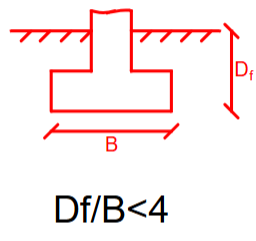
\includegraphics[width=0.3\textwidth]{FOTOS/sello_cimentacion.png}
    \caption{Sello de cimentación}
    \label{fig:9_1}    
\end{figure}

\newpage
\begin{itemize}
    \item Maquinaria sensible a deformaciones $\Delta /L < 1/750 a 1/3000$
    \item Estructuras de hormigón armado $\Delta /L < 1/500$
    \item Pórticos con diagonales $\Delta /L < 1/600$
    \item Dificultades en grúas $\Delta /L < 1/300$
    \item Inclinación visible en edificios $\Delta /L < 1/250$
    \item Daños estructurales $\Delta /L < 1/150$
\end{itemize}

\begin{figure}[h]
    \centering
    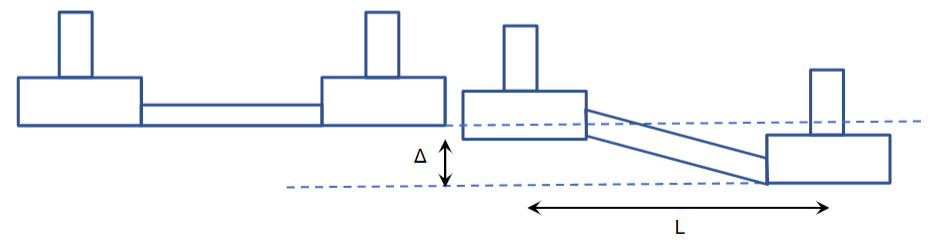
\includegraphics[width=0.5\textwidth]{FOTOS/sello_cimentacion2.png}
    \caption{Sello de cimentación}
    \label{fig:9_2}
\end{figure}

\subsection{Fundaciones profundas}
\begin{itemize}
    \item Miembros estructurales hechos de acero, hormigón o madera
    \item Sistema más costoso que fundación superficial
    \item A veces es necesario su uso para garantizar seguridad estructural:
    \begin{itemize}
        \item Transmición de cargas
        \item Esfuerzos horizontales
        \item Suelos difíciles
        \item Pilas de puentes
    \end{itemize}
\end{itemize}

\begin{figure}[h]
    \centering
    \includegraphics[width=0.3\textwidth]{FOTOS/pilotes.png}
    \caption{Pilotes}
    \label{fig:9_3}
\end{figure}

\begin{itemize}
    \item Según transmición de cargas al suelo
    \begin{itemize}
        \item Pilotes de punta
        \item Pilotes de fricción
        \item Pilotes de compactación
    \end{itemize}
    \item Según sistema constructivo
    \begin{itemize}
        \item Pilotes hincados
        \item Pilotes perforados
        \begin{itemize}
            \item Con camisa
            \item Sin camisa
        \end{itemize}
    \end{itemize}
\end{itemize}

\subsection{Fundaciones de máquinas}
\begin{itemize}
    \item Las máquinas son sensibles a los cambios de nivel o asentamientos
    \item Es conveniente usar aisladores en unión con las máquinas para evitar transmitancia de vibraciones
    \item Las fundaciones deben impedir que las vibraciones en ellas por las máquinas sean excesivas. El peso de las fundaciones puede varias de 2 a 10 veces el peso de una máquina
\end{itemize}

\subsection{Aisladas sísmicamente}
Los aisladores sísmicos friccionales consisten en un conjunto de láminas de goma natural y acero, colocadas alternadamente y adheridas entre sí, para formar un dispositivo con una gran flexibilidad horizontal y una gran rigidez vertical 

Esta tecnología puede resultar en un costo mayor al valor del edificio, que rodea entre el 3 y el 5\%. Es una buena medida especialmente para edificios en hormigón con proyección de uso de 50 años o más

\part{Capítulo 10}
\section{Consideraciones generales}
\subsection{Tipos}
\begin{itemize}
    \item Cerámica:
    \begin{itemize}
        \item Ladrillos artesanales
        \item Ladrillos prensados: macizos, perforados o huecos
        \item Mampuestros: de muros, pisos o chimeneas
    \end{itemize}
    \item Hormigón:
    \begin{itemize}
        \item Bloques llenos
        \item Bloques huecos
    \end{itemize}
    \item Piedra:
    \begin{itemize}
        \item Sillarías: piedra labrada por todas sus Características
        \item Mampuestos: piedra labrada por una sola cara
        \item Piedra bruta: sin labrar
    \end{itemize}
    \item Adobe
\end{itemize}

La unión de piezas que formen una estructura se hace mediante mortero de cemento, logrando además:
\begin{itemize}
    \item Dar resistencia al muro
    \item Lograr un sellado entre juntas
    \item Adherencia con el acero de reguerzo en las juntas, los amarres metálicos y pernos de anclaje
    \item Dar una buena calidad arquitecónica
    \item Compensar las posibles variaciones de dimensiones de los bloques
\end{itemize}

\subsection{Albañilería de cerámicos o ladrillos de arcilla}
Materia prima del ladrillo cerámico es la arcilla, el agua, y en algunos casos aditivos especiales
Características:
\begin{itemize}
    \item Facilidad de uso tanto en soluciones constructivas simples como estructurales
    \item Propiedades mecánicas y físicas favorables, como:
    \begin{itemize}
        \item Permanencia: no hay procesos químicos que lo afecten, excepto ciclos de hielo y deshielo
        \item Resistencia a la compresión
        \item Buen aislante térmico y acústico
        \item Resistencia al fuego
        \item Buena adherencia con el mortero
        \item Buena integración con otros materiales
    \end{itemize}
    \item Gran variedad de calidades y de formas
    \item Confiere con facilidad textura superficial sin terminaciones ni revestimientos adicionales
\end{itemize}

\subsubsection{Ladrillos hechos a máquina}
Fabricado por amasado, moldeado y prensado de la pasta de arcilla
\begin{itemize}
    \item Extracción y transporte
    \item Preparación
    \item moldeadoCocción en horno
\end{itemize}
\subsubsection{Ladrillos hechos a mano}
\begin{itemize}
    \item Extracción de yacimientos de arcilla
    \item Preparación de la arcilla
    \item Mezcla de agua y arcilla
    \item Amasado
    \item Moldeado
    \item Secado
    \item Cocción
\end{itemize}

\subsection{Características y Propiedades de ladrillos de arcilla}
\begin{itemize}
    \item Resistencia a la compresión
    \item Absorción de agua
    \item Adherencia a cizalle
    \item Determinación de la eflorescencia
    \item Determinación de la succión
    \item Comprobación de dimensiones
    \item Comprobación de formas
    \item Desconchamientos
    \item Fisuras
\end{itemize}
\newpage
\subsubsection{Clasificación de ladrillos cerámicos}
\begin{itemize}
    \item Clasificación por uso
    \item Clasificación por clases
    \item Clasificación por grado
\end{itemize}

\begin{figure}
    \centering
    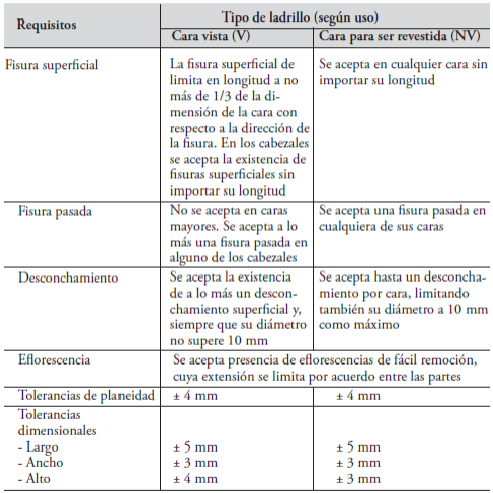
\includegraphics[width=0.5\textwidth]{FOTOS/clas_ladrillos_cer.png}
    \caption{Ladrillos}
    \label{fig:ladrillos}
\end{figure}

\begin{figure}
    \centering
    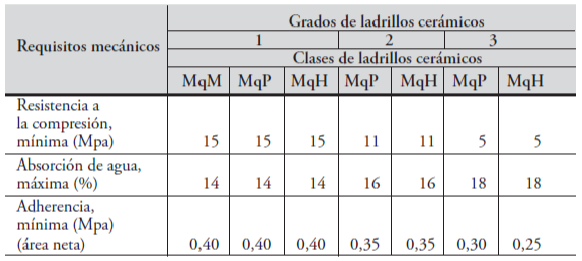
\includegraphics[width=0.5\textwidth]{FOTOS/clas_ladrillos_cer2.png}
    \caption{Ladrillos}
    \label{fig:ladrillos2}
\end{figure}

Existen tres tipos de Albañilería de ladrillo:
\begin{itemize}
    \item Albañilería simple o de relleno
    \item Albañilería armada
    \item Albañilería confinada
\end{itemize}

Muros de ladrillo:
\begin{itemize}
    \item Hilada
    \item Tendel o cantería
    \item Escantillado
\end{itemize}

\begin{figure}[h]
    \centering
    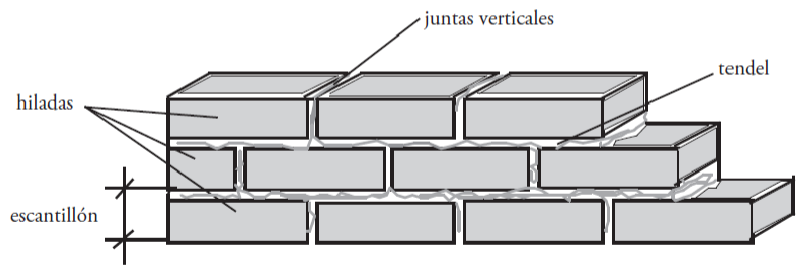
\includegraphics[width=0.5\textwidth]{FOTOS/muro_ladrillo.png}
    \caption{Muros de ladrillo}
    \label{fig:muros_ladrillo}
\end{figure}

Los aparejos más comunes son:
\begin{itemize}
    \item De Soga
    \item De Cabeza
    \item Pandereta
    \item De Sardinel
\end{itemize}

Algunas Consideraciones:
\begin{itemize}
    \item Tipo de aparejo a usar
    \item Traslapo de aparejos: se recomienda usar un traslapo de ½ si es ladrillo prensado y 1/3 si es ladrillo chonchón
\end{itemize}

Tipos de terminación del tendel o cantería:
\begin{itemize}
    \item Enrasado
    \item Rehundido
    \item Cóncavo
    \item En V
    \item Resaltado
    \item Matado (cortagotera)
\end{itemize}

Algunas Consideraciones:
\begin{itemize}
    \item Antes de colocar los ladrillos deben haber permanecido bajo agua durante 24 horas
    \item La primera hilada de ladrillos se pone de base y referencia
    \item Es necesario tener en cuenta la ubicación de vanos para puertas y ventanas
    \item Al poner las hiladas se debe conservar la altura del escantillón calculada previamente
    \item Hecha la albañilería, requiere curado que varía entre 3 y 15 días
    \item En caso de una albañilería armada, el diámetro del refuerzo vertical debe ser menor o igual a un medio de la menor dimensión del hueco en que irá inserto
    \item todos los huecos que llevan armadura de refuerzo deben llenarse con hormigón de relleno
\end{itemize}

\section{Inspección de obras}
Se eximen de los controles anteriores las viviendas individuales que cumplan simultáneamente las siguientes condiciones:
\begin{itemize}
    \item ener superficie inferior a 100 m2
    \item tener un número de pisos iguala o menor que dos
    \item ser construida bajo la supervisión directa del proyectista, quien calificará la calidad de la ejecución
    \item no formar parte de un conjunto de viviendas
\end{itemize}

\section{Albañilería de bloques de cemento}
Es más barata como solución constructiva que usando ladrillo de arcilla, pero no es más resistente
\begin{itemize}
    \item CLASE A: bloques para muros soportantes
    \item CLASE B: bloques para tabiques o muros no soportantes
\end{itemize}
La NCh 181 establece que para soporte se deben usar bloques de 190 mm o superior. Los de 140 mm se pueden usar para edificaciones de un piso o bien para divisiones interiores

\begin{itemize}
    \item Resistencia
    \item Absorción de humedad
    \item Aislación térmica
    \item Aislación acústica
    \item Resistencia al fuego
\end{itemize}

\subsection{Muros}
\begin{itemize}
    \item Albañilería simple
    \item Albañilería armada
    \item Albañilería confinada
\end{itemize}

\subsection{Consideraciones}
\begin{itemize}
    \item Mantener la verticalidad de los muros
    \item El mortero de junta debe estar fresco durante todo el tiempo de colocación
    \item La velocidad de elevación de una albañilería no debe exceder a 1.2 m. por día
    \item Las armaduras deben cumplir a las dimensiones especificadas y que no presenten óxido en escamas
    \item Todos los huecos que llevan armadura de refuerzo deben llevar hormigón de relleno
\end{itemize}

\subsection{Morteros para Albañilería}
\begin{itemize}
    \item mortero de junta
    \item mortero de relleno
    \item mortero de estuco
\end{itemize}

\end{document}
